\documentclass[twoside]{article}
\setlength{\oddsidemargin}{0.25 in}
\setlength{\evensidemargin}{-0.25 in}
\setlength{\topmargin}{-0.6 in}
\setlength{\textwidth}{6.5 in}
\setlength{\textheight}{8.5 in}
\setlength{\headsep}{0.75 in}
\setlength{\parindent}{0 in}
\setlength{\parskip}{0.1 in}

\usepackage{graphicx}
\usepackage{url}


%
% The following commands sets up the lecnum (lecture number)
% counter and make various numbering schemes work relative
% to the lecture number.
%
\newcounter{lecnum}
\renewcommand{\thepage}{\thelecnum-\arabic{page}}
\renewcommand{\thesection}{\thelecnum.\arabic{section}}
\renewcommand{\theequation}{\thelecnum.\arabic{equation}}
\renewcommand{\thefigure}{\thelecnum.\arabic{figure}}
\renewcommand{\thetable}{\thelecnum.\arabic{table}}
\newcommand{\dnl}{\mbox{}\par}

%
% The following macro is used to generate the header.
%
\newcommand{\lecture}[4]{
  \pagestyle{myheadings}
  \thispagestyle{plain}
  \newpage
  \setcounter{lecnum}{#1}
  \setcounter{page}{1}
  \noindent
  \begin{center}
  \framebox{
     \vbox{\vspace{2mm}
   \hbox to 6.28in { {\bf COMPSCI~590S~~~Systems for Data Science
                       \hfill Fall 2017} }
      \vspace{4mm}
      \hbox to 6.28in { {\Large \hfill Lecture #1: #2  \hfill} }
      \vspace{2mm}
      \hbox to 6.28in { {\it Lecturer: #3 \hfill Scribe(s): #4} }
     \vspace{2mm}}
  }
  \end{center}
  \markboth{Lecture {#1}: #2}{Lecture {#1}: #2}
  \vspace*{4mm}
}

%
% Convention for citations is authors' initials followed by the year.
% For example, to cite a paper by Leighton and Maggs you would type
% \cite{LM89}, and to cite a paper by Strassen you would type \cite{S69}.
% (To avoid bibliography problems, for now we redefine the \cite command.)
%
\renewcommand{\cite}[1]{[#1]}

% \input{epsf}

%Use this command for a figure; it puts a figure in wherever you want it.
%usage: \fig{NUMBER}{FIGURE-SIZE}{CAPTION}{FILENAME}
\newcommand{\fig}[4]{
           \vspace{0.2 in}
           \setlength{\epsfxsize}{#2}
           \centerline{\epsfbox{#4}}
           \begin{center}
           Figure \thelecnum.#1:~#3
           \end{center}
   }

% Use these for theorems, lemmas, proofs, etc.
\newtheorem{theorem}{Theorem}[lecnum]
\newtheorem{lemma}[theorem]{Lemma}
\newtheorem{proposition}[theorem]{Proposition}
\newtheorem{claim}[theorem]{Claim}
\newtheorem{corollary}[theorem]{Corollary}
\newtheorem{definition}[theorem]{Definition}
\newenvironment{proof}{{\bf Proof:}}{\hfill\rule{2mm}{2mm}}

% Some useful equation alignment commands, borrowed from TeX
\makeatletter
\def\eqalign#1{\,\vcenter{\openup\jot\m@th
 \ialign{\strut\hfil$\displaystyle{##}$&$\displaystyle{{}##}$\hfil
     \crcr#1\crcr}}\,}
\def\eqalignno#1{\displ@y \tabskip\@centering
 \halign to\displaywidth{\hfil$\displaystyle{##}$\tabskip\z@skip
   &$\displaystyle{{}##}$\hfil\tabskip\@centering
   &\llap{$##$}\tabskip\z@skip\crcr
   #1\crcr}}
\def\leqalignno#1{\displ@y \tabskip\@centering
 \halign to\displaywidth{\hfil$\displaystyle{##}$\tabskip\z@skip
   &$\displaystyle{{}##}$\hfil\tabskip\@centering
   &\kern-\displaywidth\rlap{$##$}\tabskip\displaywidth\crcr
   #1\crcr}}
\makeatother

% **** IF YOU WANT TO DEFINE ADDITIONAL MACROS FOR YOURSELF, PUT THEM HERE:



% Some general latex examples and examples making use of the
% macros follow.

\begin{document}

%FILL IN THE RIGHT INFO.
%\lecture{**LECTURE-NUMBER**}{**DATE**}{**LECTURER**}{**SCRIBE**}
\lecture{12}{Hashing, Distributed Hash Tables, and Chord}{Emery Berger}{Samuel Ginzburg}

\section{Quick Overview of HashTables}

HashTables are a data structure that seek to provide O(1) access time on average to values given a specific key. HashTables use a hashing algorithm in order to hash the keys to an offset in an array, which can then be used to lookup the value associated with the key. Since arrays are of a fixed size, and HashTables grow in size over time, HashTables cannot be static, and must be dynamic.

The hashing function used to convert the keys into offsets for looking up the value in the array should generally form a random distribution if the algorithm is good.

Typically this results in a random projection from keys to values:

\begin{center}
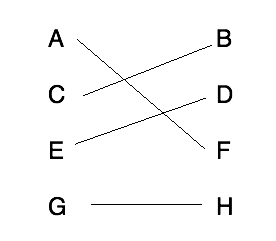
\includegraphics{randomprojection}
\end{center}

There is also the pigeonhole principle, which states that if a HashMap has M objects and N bins to place those objects in, and if M $>$ N, then some bin has more than 1 item. 

In addition to this we know that the expected length of the traversal is E$[\frac{M}{N}]$, where M is the number of objects, and N is the number of bins.

In addition, there are concurrent HashMaps, which allow for concurrent access by using locks.

There are implementations that use a singular global lock, and implementations that lock every single key with a lock, as well as implementations inbetween that form buckets and have a lock for each bucket.

Java Objects all have hashCodes via the hashCode() method derived from the Object class.

\section{Distributed Hash Tables}

The idea behind distributed hash tables is that the key-value pairs can be distributed onto multiple machines, to store particularly large hash tables.

\section{Chord}

A problem with distributed hash tables is that once they get sufficiently large, if you have to split a bucket, you will have to rehash all the values in the hash table, which is an extremely expensive operation for sufficiently large data sets. 

The Chord paper describes an algorithm for adding new nodes without having to rehash the values on every single machine.

\begin{center}
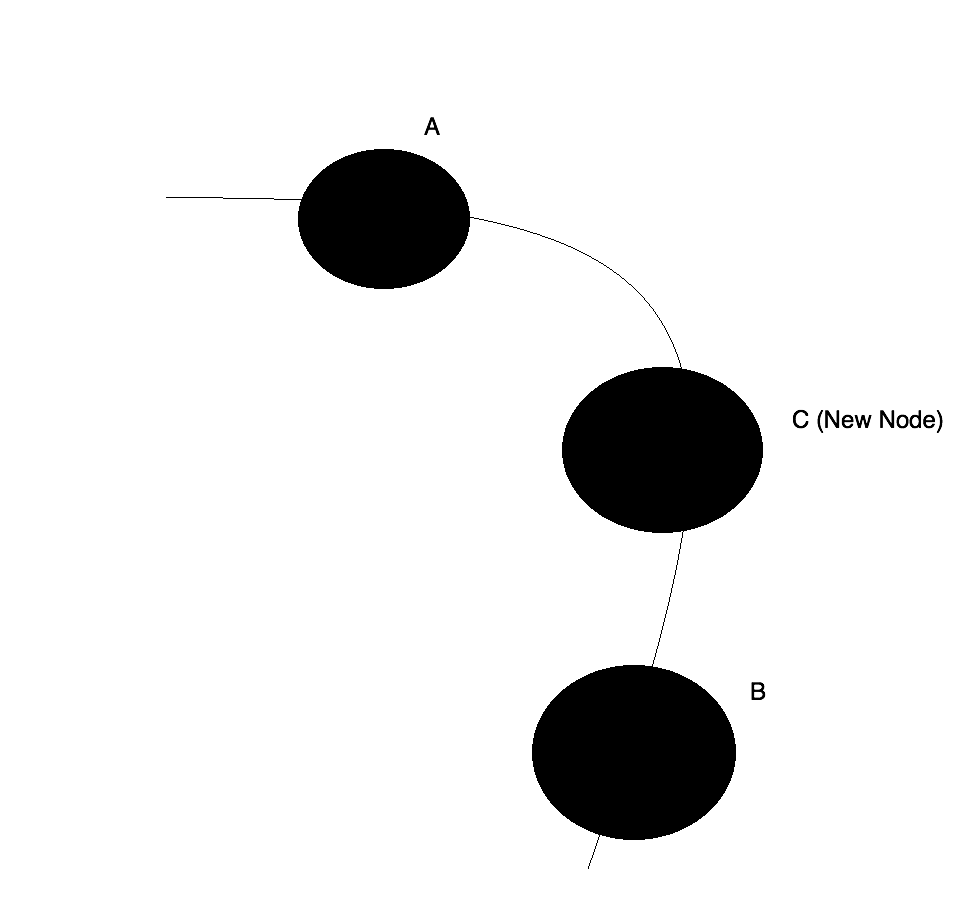
\includegraphics{chord_new_node.png}
\end{center}

In the diagram above we see that we were able to add a new node C into the chord system, and the only node that will have to be rehashed in the image above is B. This means that for each insertion of a new node, the number of rehashes is O(1), and not O(n), which would be computationally intractable for large key-value stores.

\begin{center}
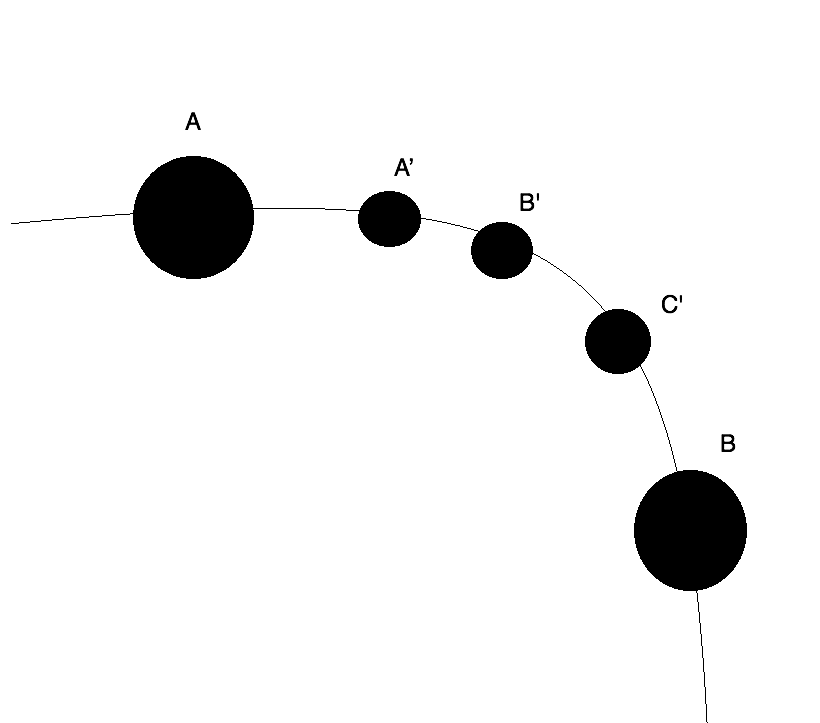
\includegraphics{chord_virtual_nodes.png}
\end{center}

In between nodes in Chord, there exist virtual nodes, which point to an actual node. The purpose of these virtual nodes is to distribute load across the system. In the example above, we see a chord system with 3 actual nodes (A, B, C), and the virtual nodes for those three nodes are distributed evenly throughout the system like the image above. 

\nocite{*}
\bibliographystyle{unsrt} 
\bibliography{ref}


\end{document}


